\subsubsection{Komplettsystem}
\begin{figure}[h!]
	\centering
	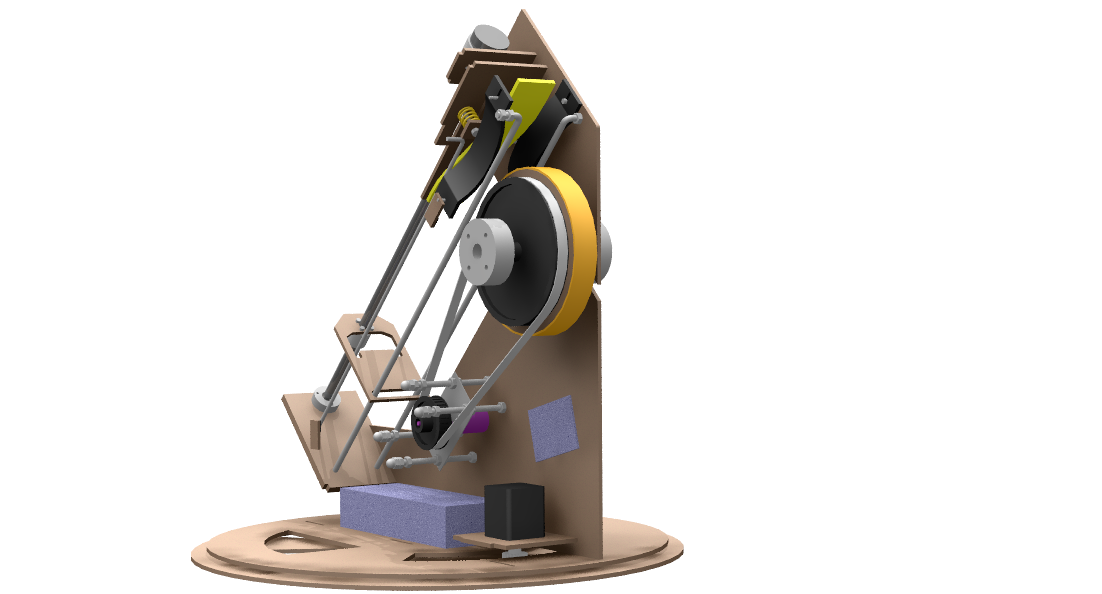
\includegraphics[width=\linewidth]{../../fig/Komplettsystem}
	\caption{Komplettsystem}
	\label{fig:Komplettsystem}
\end{figure}
\paragraph{Komponentenbeschrieb}
Das System ist in die Teilsysteme "Ausrichtung Drehturm", "Ballnachschub", "Drehturm", "Anpressvorrichtung" und "Wurfmechanismus" unterteilt, auf welche nachfolgend genauer eingegangen wird. Um die verschiedenen gelaserten Komponenten zu verbinden sind vorwiegend Steckverbindungen eingesetzt.Um dies zu ermöglichen sind den Einzelteilen Aussparungen und Nuten beigefügt. Anbaukomponenten wie Lager oder Halterungen sind mit Schraub-, sowie vereinzelt Klebeverbindungen befestigt. Die zwei Grundplatten sind mit eingepressten Alustiften verbunden.

\paragraph{Entwicklungsprozess}
Für die Entwicklung der Wurfmaschine wurden diverse Handskizzen erstellt. Nach Auswahl des Konzeptes, visualisierte und entwickelte man alle weiteren Ideen mittels dem CAD-Programm Siemens NX8 bzw. NX9. Durch dieses Vorgehen konnten Änderungen jeweils schnell angebracht werden. Bei den einzelnen Komponenten wurden bewusst nicht alle Befestigungsbohrungen im CAD-Modell erstellt, um nach dem Laserfertigen noch Spielraum für Veränderungen zu haben. Für einige mechanische Komponenten wurden detaillierte technische Zeichnungen erstellt, um sie über die schulinterne mechanische Werkstatt fertigen zu lassen.